\chapter{Data analysis}\label{ch:analysis}

To perform the analysis of the three scenarios we have prepared a shell
script\footnote{\code{simulations/simulate.sh}.} that executes parallel runs
with the configuration specified by a command line parameter and exports the
results inside a specified folder in the \code{analysis/} directory in CSV
format.

The \code{analysis/} directory contains various Jupyter notebook used to analyze
the data. Those notebooks have been developed with automation in mind: we just
need to configure it in the ``Config'' section at the start of the notebook and
run it. Python will then output a complete analysis on the provided data. This
means that, often, not all the plots/tables created by these scripts are really
useful for the analysis (they are plotted, but this does not mean they are
meaningful in every situation). Moreover, when we need to run the same Jupyter
notebook with different configuration parameters \exgratia{to apply or not a
transformation on the predicted variable in the 2\textsuperscript{k}r assumption
verification} we will just copy and paste the notebook and change the needed
configuration parameters.

The \code{analysis/} folder contains ``generic'' Jupyter notebooks that we will
copy inside some other folder before run it for a specific scenario. So, for
example, analysis for the ``High density scenario'' can be found inside the
\code{analysis/HighDensity} folder.

For each Jupyter notebook execution we have also saved the output in HTML
format. So, as an example, for the ``High density scenario'', inside the
\code{analysis/HighDensity/exported\_html/} you can found the output of each
Jupyter notebook of the \code{analysis/HighDensity/} directory. This may be
useful to inspect the results of our analysis even if Jupyter is not installed.

In the following we will discuss the most important considerations on the
results provided by Python. In any case, we will ofter refer to the Jupyter
notebook file which contains the full analysis. So, for example, if in the
``High density scenario'' we mention the \code{2kr.ipynb} file, head to the
\code{analysis/HighDensity/2kr.ipynb} file to read the full analysis (or the
equivalent HTML exported version inside the \code{exported\_html/} sub-folder).

\section{High density scenario}\label{sec:high-density}

The Jupyter notebooks used for the analysis of this scenario, along with their
output, are available inside the \code{analysis/HighDensity/} folder.

\subsection{2\texorpdfstring{\textsuperscript{k}}{k}r
analysis}\label{subsec:rect2kr}

Analysis performed with \(k\!=\!4\) and \(r\!=\!10\), for a total of \(2^4 \cdot
10 \!=\!160\) experiments. The performance indexes evaluated are the one defined
in \secref{sec:indexes}. When we talk about the total number of messages sent
remember that we are analyzing the \emph{energy efficiency} (\(\mathit{Eff}\))
of the network.

The simulation configuration for this analysis, named ``Rectangular2kr'' can be
found in the \code{simulations.ini} file. The simulations have been run using
our \code{simulate.sh} script with the following command:
\begin{verbatim}
$ ./simulate.sh -s Rectangular -c Rectangular2kr
\end{verbatim}

First, we have verified that the range of values for the \code{maxCopies}
parameter (3--7) was fine. The analysis can be found in \code{histograms.ipynb}.
Here, we just check that with \(m\!=\!3\) and \(m\!=\!7\) we get that a lot of
users decide to not relay the message in the first case and only a small bunch
of users decide to not relay the message in the second case.

Then, the 2\textsuperscript{k}r analysis can be found in \code{2kr.ipynb}. We
will verify the assumptions of normality, independence and finite variance for
the residuals in \secref{subsec:rectassumptions}. Here we will discuss the
results.

\section{Coverage}\label{sec:startnodecoverage}

File \code{coverage.ipynb} contains the histograms for the coverage obtained
with the configuration named ``StartNodePosition''. All parameters have been
fixed and we have performed 200 experiments with the starting user at the
center, border and corner --- for a total of 600 experiments.

The notebook also shows statistics about the coverage in the three cases.
Results are shown in \tableref{table:startnodecoveragestats}.

\begin{table}[hbt]
	\centering
	\begin{tabular}{lcccc}
		\toprule
		Start Node Pos\@. & Mean & Std\@. Dev\@. & Min\@. & Max\@. \\
		\midrule
		Center & \makecell[c]{\(1235.785\) \\ (\(98.942\%\))}
		       & \makecell[c]{\(7.084471\) \\ (\(0.5672\%\))}
		       & \makecell[c]{\(1213\) \\ (\(97.1177\%\))}
		       & \makecell[c]{\(1248\) \\ (\(99.9199\%\))} \\[16pt]
		Border & \makecell[c]{\(1225.345\) \\ (\(98.1061\%\))}
		       & \makecell[c]{\(123.317566\) \\ (\(9.8733\%\))}
		       & \(0\)
		       & \makecell[c]{\(1248\) \\ (\(99.9199\%\))} \\[16pt]
		Corner & \makecell[c]{\(910.64\) \\ (\(72.9095\%\))}
		       & \makecell[c]{\(546.580205\) \\ (\(43.7614\%\))}
		       & \(0\)
		       & \makecell[c]{\(1248\) \\ (\(99.9199\%\))} \\
		\bottomrule
	\end{tabular}
	\caption{Statistics about coverage when the starting node is in the
	center/border/corner (low density
	condition)}\label{table:startnodecoveragestats}
\end{table}

As we can see, the mean is higher if the starting user is positioned in the
center and lower if it is positioned in the border or corner. Additionally we
have higher standard deviations when the starting user is moved near the corner.
When the starting user is in the center, we have are able to guarantee a
coverage of at least \(97\%\) with \(R\!=\!25m\) in low density conditions,
while when the starting user is placed at the border or the corner the coverage
can drop down to zero.

Files \code{\{low,high\}-density-coverage.ipynb} contain the analysis of the
coverage in the two conditions (low density and high density) when the radius is
varied from very low values to high values. Data has been collected using the
configurations named ``StartNodePositionLowDensity'' and
``StartNodePositionHighDensity''.

\figref{subfig:ldstartnodecoverage} shows the results for the low density
case\footnote{For easier visualization, the Jupyter notebook also contains the
same data plotted in three different figures rather than with the center, border
and corner cases in the same plot.}. As we can see, in the ``center'' case the
mean coverage starts very high even with low values of \(R\): The minimum mean
is around \(1150\) (from a total of \(1249\) reachable users) and it stabilizes
near the value \(1240\) for \(R \ge 25m\).

\begin{figure}[hbt]
	\centering
	\begin{subfigure}[b]{0.49\textwidth}
		\centering
		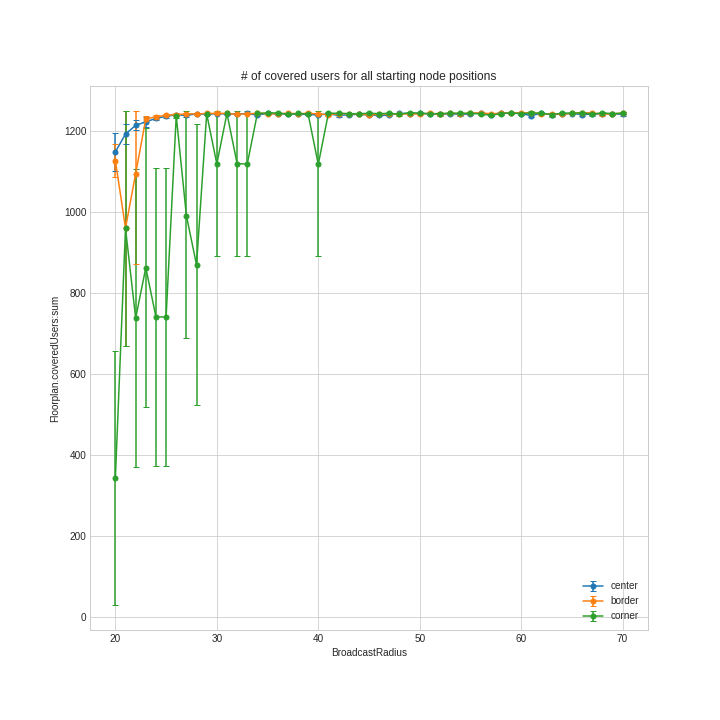
\includegraphics[width=\textwidth]{img/ld/start-node-coverage}
		\caption{Low density scenario}\label{subfig:ldstartnodecoverage}
	\end{subfigure}
	\begin{subfigure}[b]{0.49\textwidth}
		\centering
		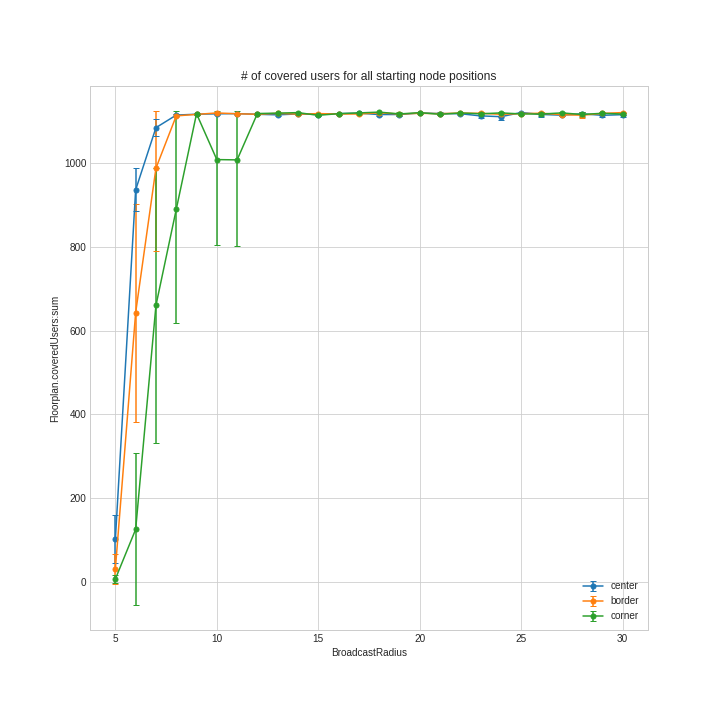
\includegraphics[width=\textwidth]{img/hd/start-node-coverage}
		\caption{High density
		scenario}\label{subfig:hdstartnodecoverage}
	\end{subfigure}
	\caption{For low values of \(R\), the coverage is generally worse if the
	starting node is in the corner rather than in the
	center}\label{fig:startnodepositioncoverage}
\end{figure}

Also in the ``border'' case the coverage stabilizes at high values with \(R \ge
25m\), but it has very high variance when the broadcast radius is very low and
it also happens that the first user sending the message is not able to reach
anyone, giving a coverage of zero.

In the ``corner'' case the situation is even worse: up until \(R \le 33m\) we
do not have a stable coverage and even after we get lower mean with a huge
variance with \(R\!=\!40m\). As we can see from the table at the end of the
notebook, this is due to a catastrophic experiment where the starting user has
not reached any user even with \(R\!=\!40m\).

\figref{subfig:hdstartnodecoverage} shows the results for the high density
scenario. Considerations are the same done for the low density scenario, so we
will not discuss the results here.

So, if possible, when designing a network of this type, to guarantee a nearly
perfect coverage, we should try to ensure that the starting user is near as much
as possible to the center or, at least, avoid the corners of the floorplan. If
this is not possible, to guarantee\footnote{With ``guarantee'' we do not mean a
100\% guarantee, of course: more experiments are needed to explore more
possibilities and, with the total randomness on the position of the users, the
only values of the broadcast radius that \emph{really} guarantees a coverage
greater than zero are those values that always make the starting user to reach
the entire floorplan immediately. Values found (\(40m\) and \(11m\)) are only an
\emph{hint} of minimum values that makes \emph{hard} to get a catastrophic
situation.} the coverage, it is necessary to increase the broadcast radius (\(R
> 40m\) for low density; \(R > 11m\) for high density).

The probability to found a user inside the area of reachability of the starting
node \idest{the probability to get a coverage greater than 0} can be easily
computed, in the general case, with~\eqref{eq:nocatastropheprobability}. The
equation has been derived by considering the inverse of the probability to found
\idest{the probability to \emph{not} found any node in the area of reachability,
which is the probability to found all the nodes in the area outside the area of
reachability} which is, for a single user, the area outside of the area of
reachability (\(X\cdot Y - \alpha\cdot\pi\cdot R^2\)) divided by the area of the
floorplan (\(X\cdot Y\)). This probability has been then extended to the case of
\(N\) users by raising it to the number of users except the first one (\(N-1\)).

\begin{equation}\label{eq:nocatastropheprobability}
	P = 1 - {\left(\frac{XY - \alpha\pi R^2}{XY}\right)}^{N-1}
\end{equation}

We can verify that for \(R\!=\!40m\), \(N\!=\!1250\), \(X\!=\!Y\!=\!500m\), with
the starting node in the corner (\(\alpha\!=\!\frac{1}{4}\)), we get:

\[
	P = 1 - {\left(\frac{500\cdot500 -
	\frac{1}{4}\pi\cdot40^2}{500\cdot500}\right)}^{1249} \simeq 99.81\%
\]

which is a quite high probability. Only in just \(\frac{1}{500}\) cases we will
get a coverage equal to zero in the case of the low density scenario with
\(R\!=\!40m\).

\subsubsection{Total number of collisions}\label{subsubsec:rect2krcollisions}

For the total number of collisions we get a very low unexplained variation
(\(0.72\%\)). The broadcast radius accounts for the \(64.31\%\) of the variation
and it is the dominant factor, as in other scenarios. As in the low density
scenario and differently from the high density one, the second most important
factor was the maximum number of copies, which accounts for the \(16.47\%\) of
the variation while the maximum relay delay (third factor) accounts only for the
\(4.86\%\) of the variation. In this case, also the combination of the broadcast
radius and the maximum number of copies is relevant (\(9.59\%\)). This results
are not surprisingly because the density of the rectangular scenario is the same
as the low density one (which is a square).

As in the case of other configurations, we need to decrease the broadcast radius
to reduce the total number of collision, which is an obvious consideration, and
as shown in \figref{fig:rectperfcollisionsm} using lower values for the maximum
number of copies reduces the total number of collisions.

The fact that the broadcast radius is less important in this scenario compared
to the high density case, but more important with respect to the low density,
can be explained by the fact that the users are scattered in the floorplan, so
we need a huger increase of the broadcast radius to see an effect, but they are
not so well distributed because they are flattened in the rectangle.

\begin{figure}[htb]
	\centering
	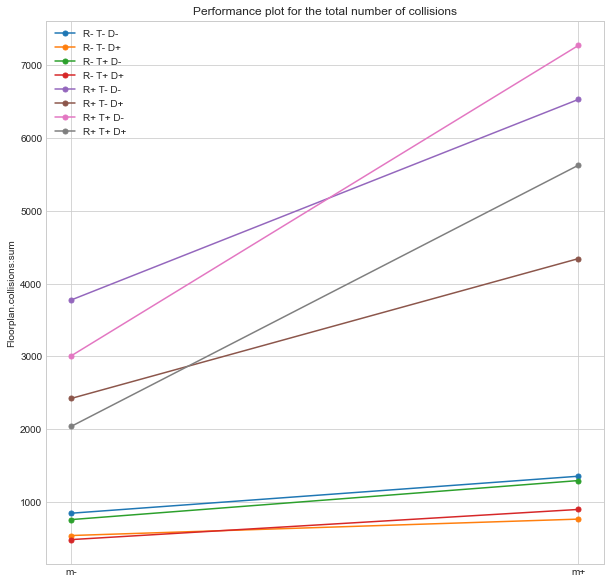
\includegraphics[width=\textwidth]{img/rect/collisions_m_perfplot.png}
	\caption{Decrease the maximum number of copies to decrease the total
	number of collisions}\label{fig:rectperfcollisionsm}
\end{figure}

\subsubsection{Total number of messages sent}\label{subsubsec:hd2krmessages}

This is an indication of the energy efficiency of the entire network.

The maximum number of copies is the dominant factor (\(85.98\%\)), as expected.
Also the broadcast radius \(R\) and its combination with the maximum
number of copies have a valuable impact on this index. The unexplained variation
is very low (\(0.53\%\)).

In \figref{subfig:hdperfmessagesm} we see that the total number of messages sent
decreases with an lower value of the \code{maxCopies} parameter, as expected.
We note that with \(m\!=\!6\) we get that nearly all the users of the network
relay the message. In \figref{subfig:hdperfmessagesR} we can see that less
messages are sent if an higher broadcast radius is used when \(m\!=\!2\). So,
with a low \(m\), we can further decrease the total number of messages sent by
increasing \(R\). Of course increasing the broadcast radius is not good for our
purpose to optimize the energy efficiency of the network, but as we can see from
\figref{subfig:hdperfmessagesT}, the same consideration made for \(R\) are also
valid for the hear window size \(T\). We perhaps expect \(T\) to hugely affect
the total broadcast time, so the selection of the factor \(T\) is a trade-off
between the energy efficiency and the total broadcast time.

\begin{figure}[hbt]
	\centering
	\begin{subfigure}[b]{0.33\textwidth}
		\centering
		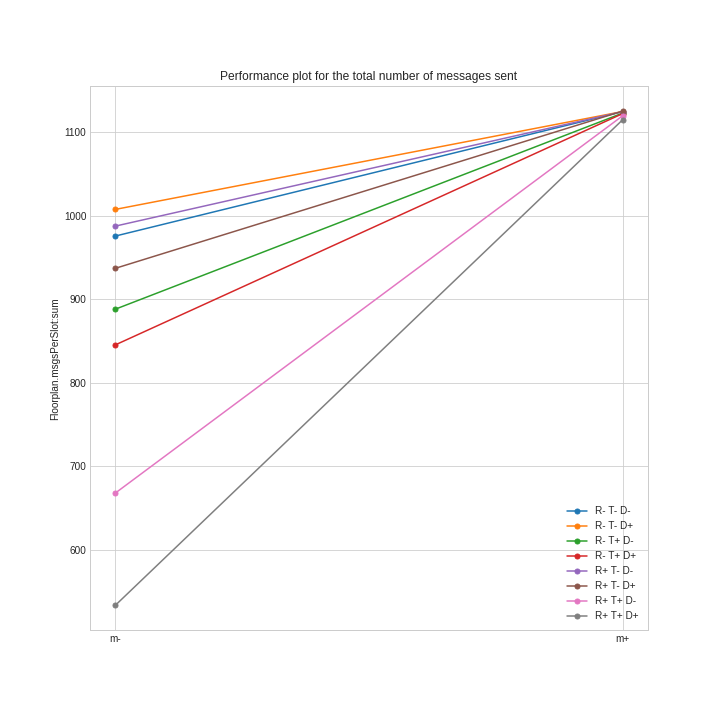
\includegraphics[width=\textwidth]{img/hd/messages-m-perfplot}
		\caption{When the maximum number of copies is reduced the total
		number of messages sent decreases}\label{subfig:hdperfmessagesm}
	\end{subfigure}
	\begin{subfigure}[b]{0.33\textwidth}
		\centering
		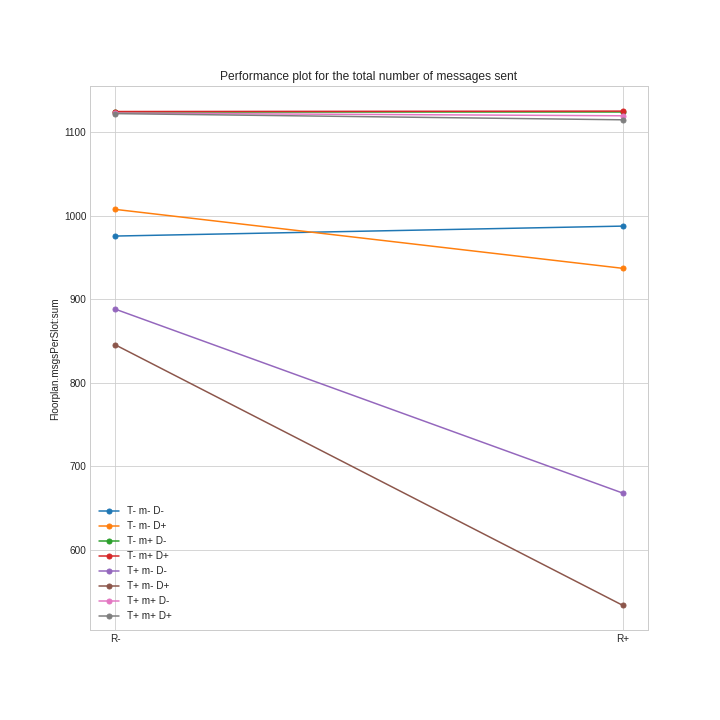
\includegraphics[width=\textwidth]{img/hd/messages-R-perfplot}
		\caption{Increase the broadcast radius when \(m\) is low to
		reduce the total number of messages
		sent}\label{subfig:hdperfmessagesR}
	\end{subfigure}
	\begin{subfigure}[b]{0.32\textwidth}
		\centering
		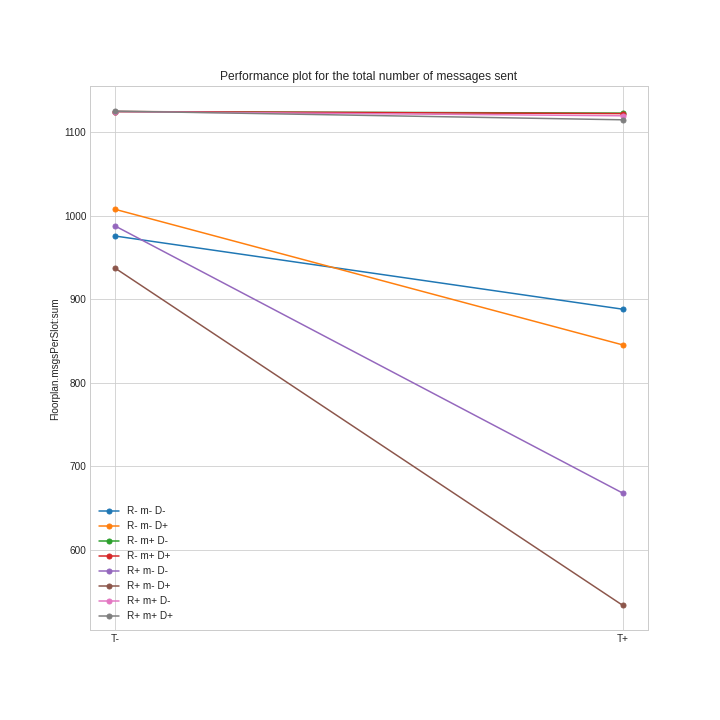
\includegraphics[width=\textwidth]{img/hd/messages-T-perfplot}
		\caption{Increase the size of the hear window when \(m\) is low
		to reduce the total number of messages
		sent}\label{subfig:hdperfmessagesT}
	\end{subfigure}
	\caption{Performance plots for the total number of messages
	sent}\label{fig:hdperfmessages}
\end{figure}

\subsubsection{Broadcast time}\label{subsubsec:hd2krtime}

Since in all the experiments we have always reached a coverage of at least
\(99\%\), here we will only discuss the broadcast time needed to reach the 99th
percentile of the coverage.

We have a large unexplained variation (\(7.95\%\)). The reason for this result
will be discussed in \chref{ch:starting-node}.

We can see that the most important factor is the broadcast radius that accounts
for the \(71.25\%\) of the variation, followed by the size of the hear window
(\(19.30\%\)). Other factors and their combinations are irrelevant. We note that
these variations are much larger than the unexplained variation, so we can still
say that they are significant. Of course, their \(95\%\) confidence intervals
also gets larger: (\(63.62\%\), \(79.30\%\)) for \(R\) and (\(15.43\%\),
\(23.59\%\)) for \(T\), but they do not include the zero.

This means that we can reduce the broadcast time by increasing the broadcast
radius to let the relayed messages to reach more user. Also the size of the hear
window can be decreased in order to reduce the time that each user wait before
deciding to relay or not relay the message. Of course, as stated before,
reducing the size of the hear window has a negative impact on the energy
efficiency, so some trade-off considerations are required.

We note that we have performed a \emph{logarithmic transformation of the
predicted variable} \idest{the total broadcast time} in order to meet the
assumption of finite variance for the residuals, as discussed in
\secref{subsec:hdassumptions}. This means that the final approximated regression
model for the broadcast time is transformed into the one shown
in~\eqref{eq:hdtimelogregressionmodel}, with \(R\) and \(T\) normalized between
\(-1\) and \(1\). (factors with low influence are removed; 95\% confidence
intervals are show in parenthesis).

\begin{equation}\label{eq:hdtimelogregressionmodel}
	\begin{cases}
		\log(t_B) = q_0 + q_R \cdot R + q_T \cdot T + e\\
		q_0 = 4.782874\\
		q_R = -0.462452 & (-0.487897, -0.437006)\\
		q_T = 0.240663 & (0.215217, 0.266109)
	\end{cases}
\end{equation}

We can then predict the total broadcast time using the formula shown
in~\eqref{eq:hdtimeregressionmodel}.

\begin{equation}\label{eq:hdtimeregressionmodel}
	t_B = e^{4.782874 - 0.462452 \cdot R + 0.240663 \cdot T}
\end{equation}

And the 95\% confidence interval as shown in~\eqref{eq:hdtimeregressionci}.

\begin{equation}\label{eq:hdtimeregressionci}
	\begin{cases}
		t^-_B = e^{4.782874 - 0.487897 \cdot R + 0.215217 \cdot T}\\
		t^+_B = e^{4.782874 - 0.437006 \cdot R + 0.266109 \cdot T}\\
	\end{cases}
\end{equation}


\subsection{Testing the assumptions}\label{subsec:hdassumptions}

The assumptions of normality, independency and finite variance must be verified
for the residuals of the observations. The complete analysis can be found in
\code{2kr-assumptions-tests.ipynb}.

\subsubsection{Normality}\label{subsubsec:rectassumptionsnormality}

In this case, we get worse results for normality compared to those obtained in
the other scenarios, with generally lower \(R^2\) and few outliers in collisions
and in messages, but we can say anyway that the normality assumption is
verified, except to the covered users, but since we do not study this index, we
do not need to get it verified.

\subsubsection{Independency}\label{subsubsec:hdassumptionsindependency}

Independency is assumed by the way we have conducted the experiments. Anyway,
the scatter plots do not show any trend.

\subsubsection{Finite variance}\label{rectassumptionsvariance}

In the collision and messages plots we haven't trends but the behaviour is
blockwise, as we can see for example in \figref{fig:recttimevariance} with
swinging results and also in this case the order of magnitude of the residual is
lower than the one of the average predicted response, so we can conclude that
the assumption of finite variance is still valid.

As for other scenarios, to verify the assumption for the residuals of the 99th
percentile of the total broadcast time we need to perform a logarithmic
transformation of the predicted variable. The result is shown in
\figref{fig:recttimevariance}.

\begin{figure}[htb]
	\centering
	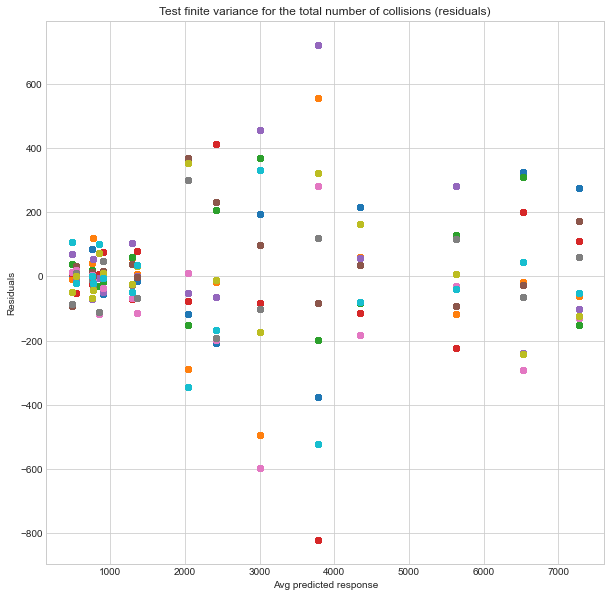
\includegraphics[width=0.6\textwidth]{img/rect/collisionvariance.png}
	\caption{Scatter plot of the variance of the residuals of the
	collisions. No trends but blockwise
	behaviour}\label{fig:recttimevariance}
\end{figure}


\subsection{Optimization for the low density
scenario}\label{subsec:ldoptimization}

The situation is the same of the high density scenario. We have run a full
factorial analysis, with low values of each parameter, in order to identify the
minimum values required to reach the coverage. Each possible configuration
(\(750\)) has been run with 10 repetitions. The complete analysis can be found
in \code{coverage.ipynb}. The configuration used is named
``LowDensityCoverage''. We have found out that to reach at least the \(99\%\) of
the coverage, we need to have a broadcast radius of at least \(23m\), but we
also need higher values for \(m\) and \(D\). If we use \(R\!=\!25m\) we get
better results for the other parameters. In particular, we have found the
following minimum configuration the we consider ``good'' and ``well balanced''
since it does not use the value \code{1} for any of the parameters.

\begin{center}
	\begin{tabular}{cccc}
		\toprule
		R & T & m & \(\max(\delta)\) \\
		\midrule
		\(25m\) & \(2s\) & \(2\,\mathit{copies}\) & \(2s\) \\
		\bottomrule
	\end{tabular}
\end{center}

If we want to optimize the \standout{total broadcast time}, as we have seen in
\secref{subsec:hd2kr}, we need to increase the broadcast radius or decrease the
size of the hear window. File \code{broadcast-time.ipynb} shows the results with
various combination of these two factors. The configuration used is named
``LowDensityTime''. We use an high value for the maximum number of copies,
since from the plot generated by the \code{2kr.ipynb} script we see a slightly
decrease of the broadcast time with high values for \(m\). For the same reason,
we use a low value for the maximum relay delay. \figref{fig:hdtimeff} shows the
result of the analysis. As we can see, by using low values for \(T\) we can get
lower values for the broadcast time, even with higher values for the broadcast
radius. So, to not sacrifice the energy efficiency, we can lower the size of the
hear window rather than increase the broadcast radius to reduce the broadcast
time.

\begin{figure}
	\centering
	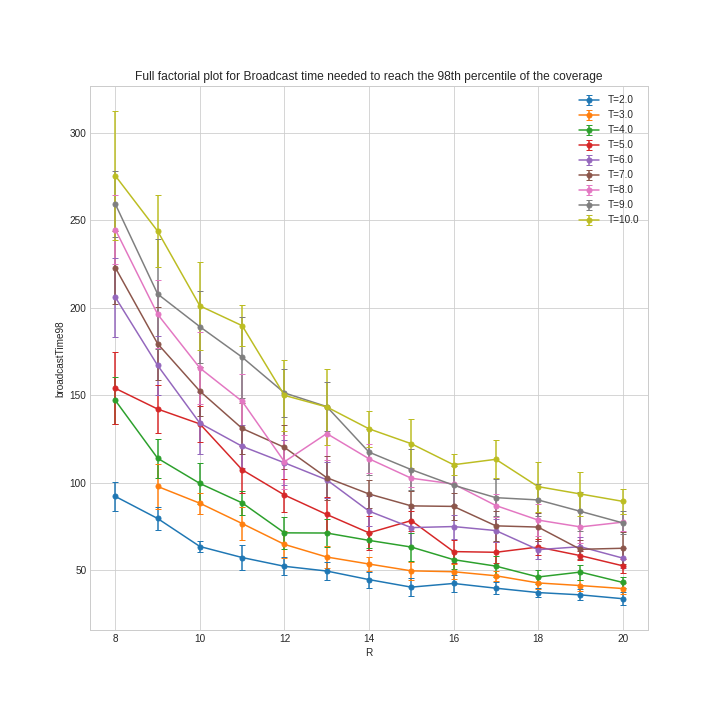
\includegraphics[width=\textwidth]{img/hd/broadcasttime-R-ffplot}
	\caption{The broadcast time is lower with higher values of the broadcast
	radius and lower values of the size of the hear
	window (95\% confidence intervals)}\label{fig:ldtimeff}
\end{figure}

We can verify that the model derived with the \(2^{k}r\) analysis is valid. If we
compute, for example, the value for \(R\!=\!17m\) and \(T\!=\!10s\) using the
model we get the result shown in~\eqref{eq:hdtimepredictionexample} (values for
the two parameters are normalized between \(-1\) and \(1\)) which is near the
mean value obtained from the full factorial analysis (\(117.2s\)) and inside its
95\% confidence interval (\(106.7255\), \(127.6745\)).

\begin{equation}\label{eq:ldtimepredictionexample}
	t_B = e^{4.782874 - 0.462452 \cdot 0.4 + 0.240663 \cdot 1} =
	e^{4.8385562} \simeq 126.2869s
\end{equation}

If instead we want to optimize the \standout{energy efficiency}, we must reduce
the broadcast radius and the total number of messages sent. In file
\code{messages.ipynb} we have performed a factorial analysis with low values for
the broadcast radius. Other factors taken into considerations are the one we
have identified as relevant in \secref{subsec:hd2kr}, namely the maximum number
of copies and the size of the hear window. The configuration used is named
``LowDensityMessages''.

As we can see from \figref{fig:hdmessagesff}, we get that the maximum number of
copies hugely affects the total number of messages sent, as previously found by
the \(2^{k}r\) analysis. Surprisingly, the combination of the maximum number of
copies and the size of the hear window is very important to reduce the number of
messages sent (the lower lines in the plot are those with the higher values for
\(T\)). This contradicts what the \(2^{k}r\) analysis found before.

\begin{figure}
	\centering
	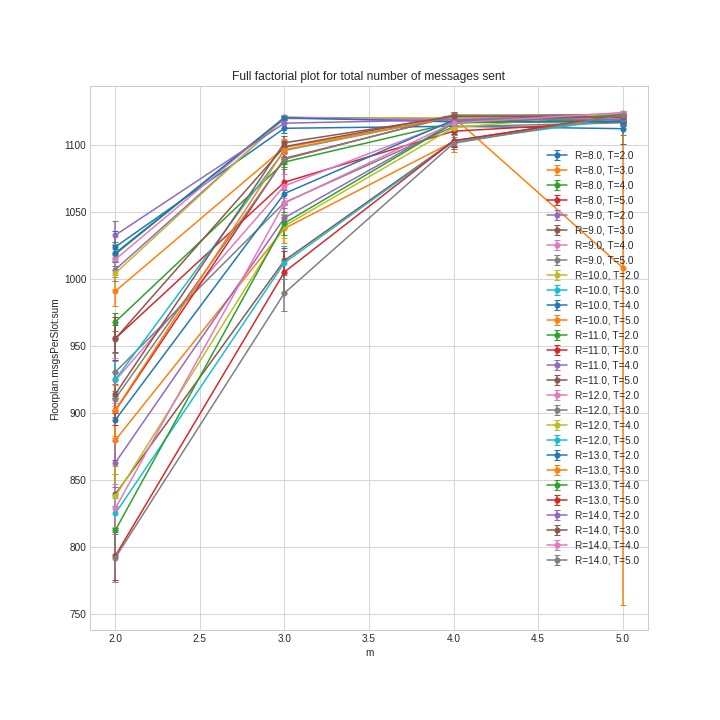
\includegraphics[width=\textwidth]{img/hd/messages-m-ffplot}
	\caption{With low values of the maximum number of copies and higher
	values for the size of the hear window, we get a lower number of
	messages sent}\label{fig:ldmessagesff}
\end{figure}

So, in order to improve the energy efficiency, since we can not increase the
broadcast radius, we need to use a large \(T\) and a low \(m\). Increasing
\(T\) also increases the broadcast time, so a trade-off decision is needed in
this parameter. In order to account for both the indexes, one can increase the
value of \(R\) to reduce the broadcast radius and increase \(T\) maintaining a
low \(m\) in order to compensate for the increment of the energy consumption due
to the higher value of \(R\).

Regarding the \standout{total number of collisions}, we can reduce it by
reducing the broadcast radius and the maximum number of copies. Also helps
increasing the maximum relay delay. If the energy efficiency is the main
performance index that we want to optimize, the best way to reduce the total
number of collisions is certainly to reduce the broadcast radius. If instead we
want to optimize the broadcast time, we can reduce the total number of
collisions by reducing \(m\) and increasing \(\max(\delta)\). Factorial
analysis with the \(m\) and \(\max(\delta)\) parameters is available in
\code{collisions.ipynb}, using the configuration named
``LowDensityCollisions''. \figref{fig:hdcollisionsff} shows the results: the
plot is very well linear in the \(\max(\delta)\) parameter, suggesting that
increasing this factor even more should allow to have even a lower number of
collisions. \(m\!=\!2\) is a good setup for this parameter since it allows to
completely exploit the advantages of the \emph{trickle relaying} algorithm in
order to reduce the number of collisions and the number of messages sent.

\begin{figure}
	\centering
	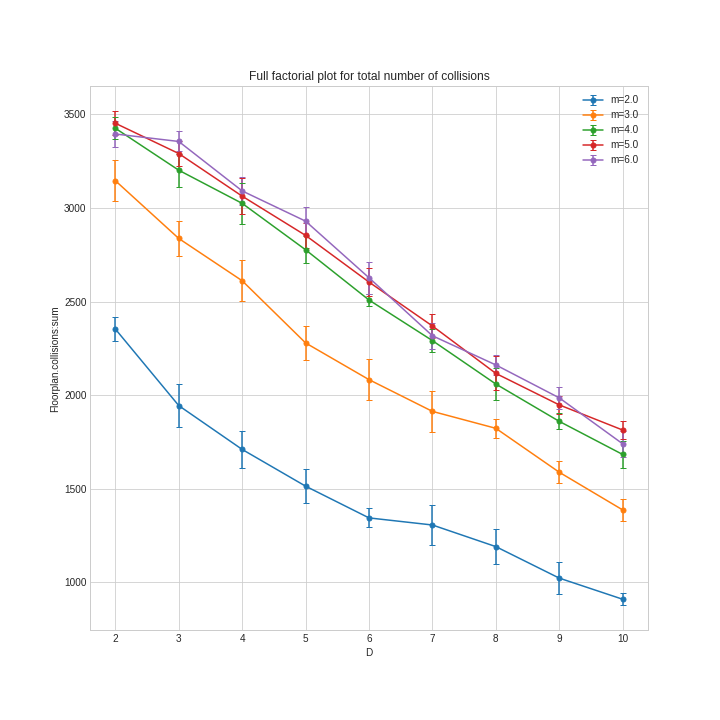
\includegraphics[width=\textwidth]{img/hd/collisions-D-ffplot}
	\caption{The number of collisions is linearly dependent on the maximum
	relay delay. Also, trickle relaying can be exploited with low values of
	\(m\) in order to reduce the number of
	collisions}\label{fig:ldcollisionsff}
\end{figure}

\subsubsection{Conclusions}\label{subsubsec:ldconclusions}

\begin{itemize}
	\item The minimal configuration to get a nearly perfect coverage is with
		\(R\!=\!8m\), \(T\!=\!2s\), \(m\!=\!2\) and
		\(\max(\delta)\!=\!2s\). Higher values for these parameters does
		not break the coverage.
	\item If a low total broadcast time is a main objective, increasing
		\(R\) is effective. Also reducing \(T\) allows for further
		improvement of the broadcast time.
	\item If instead a better energy efficiency is the main objective, \(R\)
		can not be increased and \(T\) should not be reduced. A
		trade-off decision between a low broadcast time and a good
		energy efficiency is needed.
	\item There is no reason to use large values for the maximum number of
		copies: \(m\!=\!2\) is a good set for this parameter and it
		leads to a lower number of collisions and a better energy
		efficiency without sacrificing the broadcast time. Trickle
		relaying is very effective in this job.
	\item \(\max(\delta)\) should be sufficiently high, in order to reduce
		the total number of collisions, but not too high, in order to
		avoid an increase in the broadcast time due to users waiting too
		much before relaying the message.
\end{itemize}


\section{Low density scenario}\label{sec:low-density}

\subsection{2\texorpdfstring{\textsuperscript{k}}{k}r
analysis}\label{subsec:rect2kr}

Analysis performed with \(k\!=\!4\) and \(r\!=\!10\), for a total of \(2^4 \cdot
10 \!=\!160\) experiments. The performance indexes evaluated are the one defined
in \secref{sec:indexes}. When we talk about the total number of messages sent
remember that we are analyzing the \emph{energy efficiency} (\(\mathit{Eff}\))
of the network.

The simulation configuration for this analysis, named ``Rectangular2kr'' can be
found in the \code{simulations.ini} file. The simulations have been run using
our \code{simulate.sh} script with the following command:
\begin{verbatim}
$ ./simulate.sh -s Rectangular -c Rectangular2kr
\end{verbatim}

First, we have verified that the range of values for the \code{maxCopies}
parameter (3--7) was fine. The analysis can be found in \code{histograms.ipynb}.
Here, we just check that with \(m\!=\!3\) and \(m\!=\!7\) we get that a lot of
users decide to not relay the message in the first case and only a small bunch
of users decide to not relay the message in the second case.

Then, the 2\textsuperscript{k}r analysis can be found in \code{2kr.ipynb}. We
will verify the assumptions of normality, independence and finite variance for
the residuals in \secref{subsec:rectassumptions}. Here we will discuss the
results.

\section{Coverage}\label{sec:startnodecoverage}

File \code{coverage.ipynb} contains the histograms for the coverage obtained
with the configuration named ``StartNodePosition''. All parameters have been
fixed and we have performed 200 experiments with the starting user at the
center, border and corner --- for a total of 600 experiments.

The notebook also shows statistics about the coverage in the three cases.
Results are shown in \tableref{table:startnodecoveragestats}.

\begin{table}[hbt]
	\centering
	\begin{tabular}{lcccc}
		\toprule
		Start Node Pos\@. & Mean & Std\@. Dev\@. & Min\@. & Max\@. \\
		\midrule
		Center & \makecell[c]{\(1235.785\) \\ (\(98.942\%\))}
		       & \makecell[c]{\(7.084471\) \\ (\(0.5672\%\))}
		       & \makecell[c]{\(1213\) \\ (\(97.1177\%\))}
		       & \makecell[c]{\(1248\) \\ (\(99.9199\%\))} \\[16pt]
		Border & \makecell[c]{\(1225.345\) \\ (\(98.1061\%\))}
		       & \makecell[c]{\(123.317566\) \\ (\(9.8733\%\))}
		       & \(0\)
		       & \makecell[c]{\(1248\) \\ (\(99.9199\%\))} \\[16pt]
		Corner & \makecell[c]{\(910.64\) \\ (\(72.9095\%\))}
		       & \makecell[c]{\(546.580205\) \\ (\(43.7614\%\))}
		       & \(0\)
		       & \makecell[c]{\(1248\) \\ (\(99.9199\%\))} \\
		\bottomrule
	\end{tabular}
	\caption{Statistics about coverage when the starting node is in the
	center/border/corner (low density
	condition)}\label{table:startnodecoveragestats}
\end{table}

As we can see, the mean is higher if the starting user is positioned in the
center and lower if it is positioned in the border or corner. Additionally we
have higher standard deviations when the starting user is moved near the corner.
When the starting user is in the center, we have are able to guarantee a
coverage of at least \(97\%\) with \(R\!=\!25m\) in low density conditions,
while when the starting user is placed at the border or the corner the coverage
can drop down to zero.

Files \code{\{low,high\}-density-coverage.ipynb} contain the analysis of the
coverage in the two conditions (low density and high density) when the radius is
varied from very low values to high values. Data has been collected using the
configurations named ``StartNodePositionLowDensity'' and
``StartNodePositionHighDensity''.

\figref{subfig:ldstartnodecoverage} shows the results for the low density
case\footnote{For easier visualization, the Jupyter notebook also contains the
same data plotted in three different figures rather than with the center, border
and corner cases in the same plot.}. As we can see, in the ``center'' case the
mean coverage starts very high even with low values of \(R\): The minimum mean
is around \(1150\) (from a total of \(1249\) reachable users) and it stabilizes
near the value \(1240\) for \(R \ge 25m\).

\begin{figure}[hbt]
	\centering
	\begin{subfigure}[b]{0.49\textwidth}
		\centering
		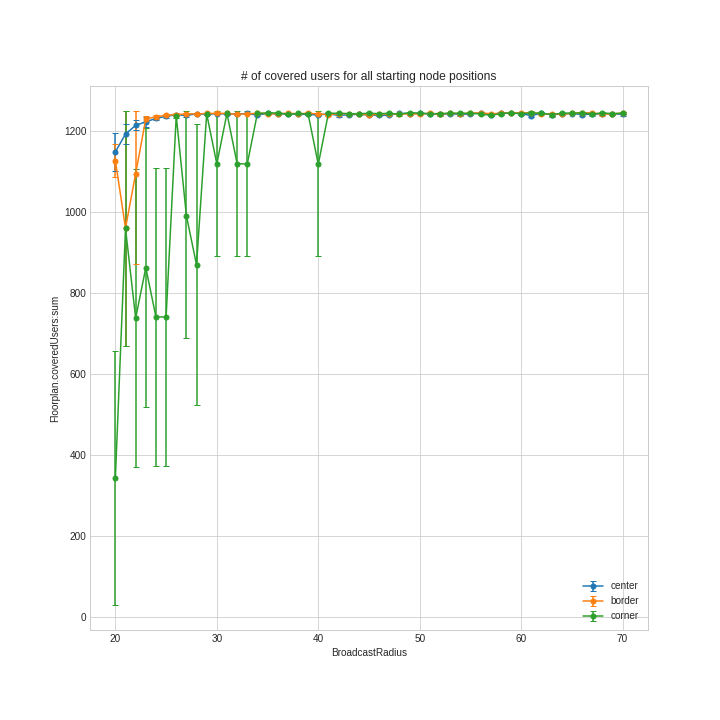
\includegraphics[width=\textwidth]{img/ld/start-node-coverage}
		\caption{Low density scenario}\label{subfig:ldstartnodecoverage}
	\end{subfigure}
	\begin{subfigure}[b]{0.49\textwidth}
		\centering
		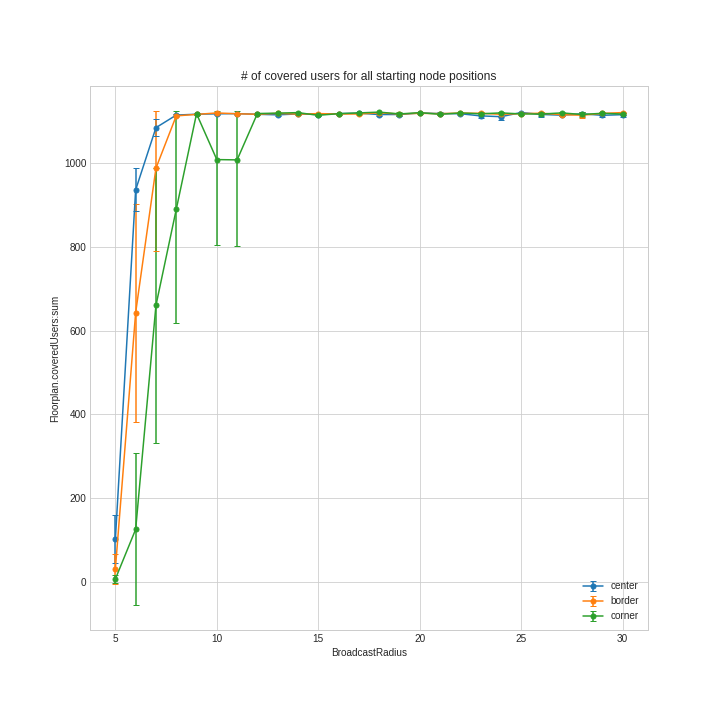
\includegraphics[width=\textwidth]{img/hd/start-node-coverage}
		\caption{High density
		scenario}\label{subfig:hdstartnodecoverage}
	\end{subfigure}
	\caption{For low values of \(R\), the coverage is generally worse if the
	starting node is in the corner rather than in the
	center}\label{fig:startnodepositioncoverage}
\end{figure}

Also in the ``border'' case the coverage stabilizes at high values with \(R \ge
25m\), but it has very high variance when the broadcast radius is very low and
it also happens that the first user sending the message is not able to reach
anyone, giving a coverage of zero.

In the ``corner'' case the situation is even worse: up until \(R \le 33m\) we
do not have a stable coverage and even after we get lower mean with a huge
variance with \(R\!=\!40m\). As we can see from the table at the end of the
notebook, this is due to a catastrophic experiment where the starting user has
not reached any user even with \(R\!=\!40m\).

\figref{subfig:hdstartnodecoverage} shows the results for the high density
scenario. Considerations are the same done for the low density scenario, so we
will not discuss the results here.

So, if possible, when designing a network of this type, to guarantee a nearly
perfect coverage, we should try to ensure that the starting user is near as much
as possible to the center or, at least, avoid the corners of the floorplan. If
this is not possible, to guarantee\footnote{With ``guarantee'' we do not mean a
100\% guarantee, of course: more experiments are needed to explore more
possibilities and, with the total randomness on the position of the users, the
only values of the broadcast radius that \emph{really} guarantees a coverage
greater than zero are those values that always make the starting user to reach
the entire floorplan immediately. Values found (\(40m\) and \(11m\)) are only an
\emph{hint} of minimum values that makes \emph{hard} to get a catastrophic
situation.} the coverage, it is necessary to increase the broadcast radius (\(R
> 40m\) for low density; \(R > 11m\) for high density).

The probability to found a user inside the area of reachability of the starting
node \idest{the probability to get a coverage greater than 0} can be easily
computed, in the general case, with~\eqref{eq:nocatastropheprobability}. The
equation has been derived by considering the inverse of the probability to found
\idest{the probability to \emph{not} found any node in the area of reachability,
which is the probability to found all the nodes in the area outside the area of
reachability} which is, for a single user, the area outside of the area of
reachability (\(X\cdot Y - \alpha\cdot\pi\cdot R^2\)) divided by the area of the
floorplan (\(X\cdot Y\)). This probability has been then extended to the case of
\(N\) users by raising it to the number of users except the first one (\(N-1\)).

\begin{equation}\label{eq:nocatastropheprobability}
	P = 1 - {\left(\frac{XY - \alpha\pi R^2}{XY}\right)}^{N-1}
\end{equation}

We can verify that for \(R\!=\!40m\), \(N\!=\!1250\), \(X\!=\!Y\!=\!500m\), with
the starting node in the corner (\(\alpha\!=\!\frac{1}{4}\)), we get:

\[
	P = 1 - {\left(\frac{500\cdot500 -
	\frac{1}{4}\pi\cdot40^2}{500\cdot500}\right)}^{1249} \simeq 99.81\%
\]

which is a quite high probability. Only in just \(\frac{1}{500}\) cases we will
get a coverage equal to zero in the case of the low density scenario with
\(R\!=\!40m\).

\subsubsection{Total number of collisions}\label{subsubsec:rect2krcollisions}

For the total number of collisions we get a very low unexplained variation
(\(0.72\%\)). The broadcast radius accounts for the \(64.31\%\) of the variation
and it is the dominant factor, as in other scenarios. As in the low density
scenario and differently from the high density one, the second most important
factor was the maximum number of copies, which accounts for the \(16.47\%\) of
the variation while the maximum relay delay (third factor) accounts only for the
\(4.86\%\) of the variation. In this case, also the combination of the broadcast
radius and the maximum number of copies is relevant (\(9.59\%\)). This results
are not surprisingly because the density of the rectangular scenario is the same
as the low density one (which is a square).

As in the case of other configurations, we need to decrease the broadcast radius
to reduce the total number of collision, which is an obvious consideration, and
as shown in \figref{fig:rectperfcollisionsm} using lower values for the maximum
number of copies reduces the total number of collisions.

The fact that the broadcast radius is less important in this scenario compared
to the high density case, but more important with respect to the low density,
can be explained by the fact that the users are scattered in the floorplan, so
we need a huger increase of the broadcast radius to see an effect, but they are
not so well distributed because they are flattened in the rectangle.

\begin{figure}[htb]
	\centering
	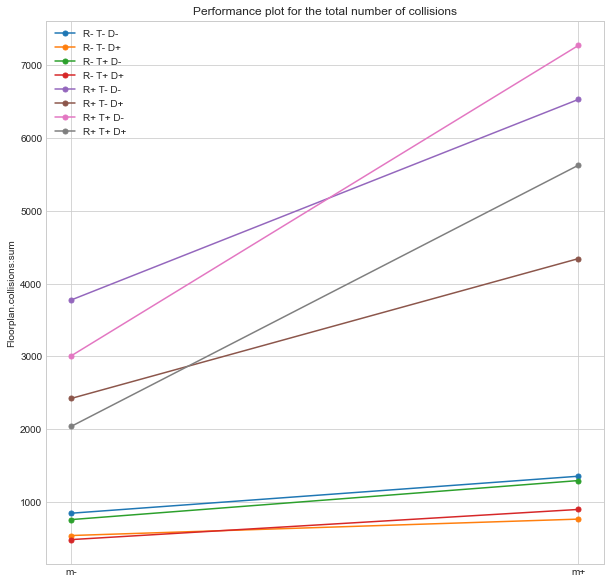
\includegraphics[width=\textwidth]{img/rect/collisions_m_perfplot.png}
	\caption{Decrease the maximum number of copies to decrease the total
	number of collisions}\label{fig:rectperfcollisionsm}
\end{figure}

\subsubsection{Total number of messages sent}\label{subsubsec:hd2krmessages}

This is an indication of the energy efficiency of the entire network.

The maximum number of copies is the dominant factor (\(85.98\%\)), as expected.
Also the broadcast radius \(R\) and its combination with the maximum
number of copies have a valuable impact on this index. The unexplained variation
is very low (\(0.53\%\)).

In \figref{subfig:hdperfmessagesm} we see that the total number of messages sent
decreases with an lower value of the \code{maxCopies} parameter, as expected.
We note that with \(m\!=\!6\) we get that nearly all the users of the network
relay the message. In \figref{subfig:hdperfmessagesR} we can see that less
messages are sent if an higher broadcast radius is used when \(m\!=\!2\). So,
with a low \(m\), we can further decrease the total number of messages sent by
increasing \(R\). Of course increasing the broadcast radius is not good for our
purpose to optimize the energy efficiency of the network, but as we can see from
\figref{subfig:hdperfmessagesT}, the same consideration made for \(R\) are also
valid for the hear window size \(T\). We perhaps expect \(T\) to hugely affect
the total broadcast time, so the selection of the factor \(T\) is a trade-off
between the energy efficiency and the total broadcast time.

\begin{figure}[hbt]
	\centering
	\begin{subfigure}[b]{0.33\textwidth}
		\centering
		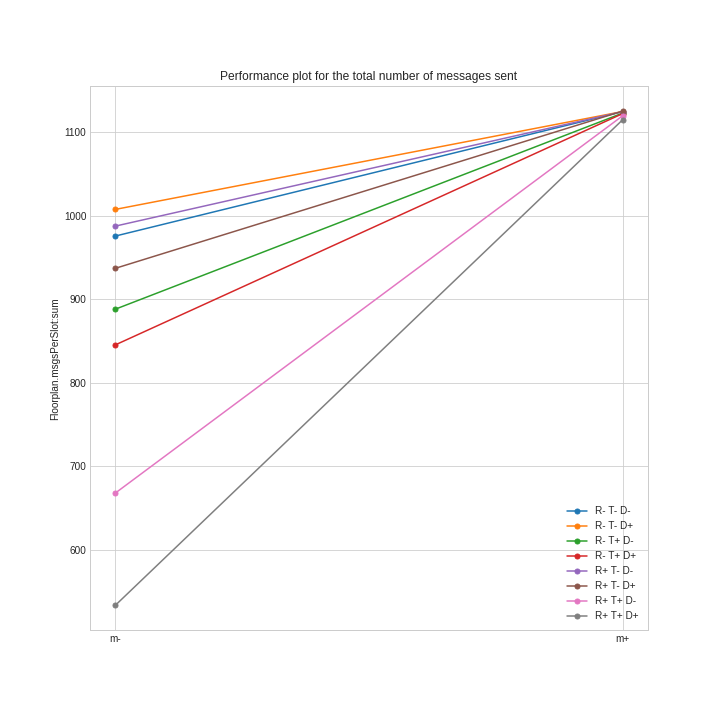
\includegraphics[width=\textwidth]{img/hd/messages-m-perfplot}
		\caption{When the maximum number of copies is reduced the total
		number of messages sent decreases}\label{subfig:hdperfmessagesm}
	\end{subfigure}
	\begin{subfigure}[b]{0.33\textwidth}
		\centering
		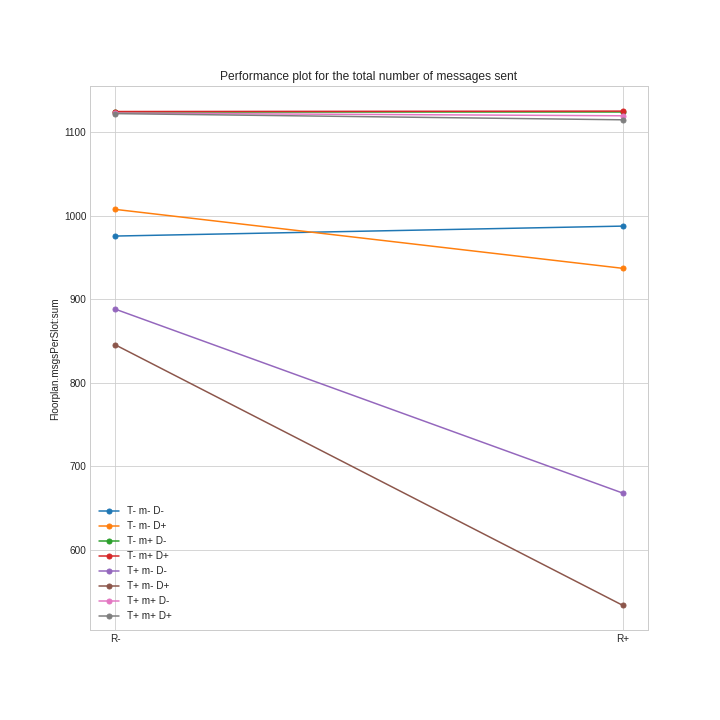
\includegraphics[width=\textwidth]{img/hd/messages-R-perfplot}
		\caption{Increase the broadcast radius when \(m\) is low to
		reduce the total number of messages
		sent}\label{subfig:hdperfmessagesR}
	\end{subfigure}
	\begin{subfigure}[b]{0.32\textwidth}
		\centering
		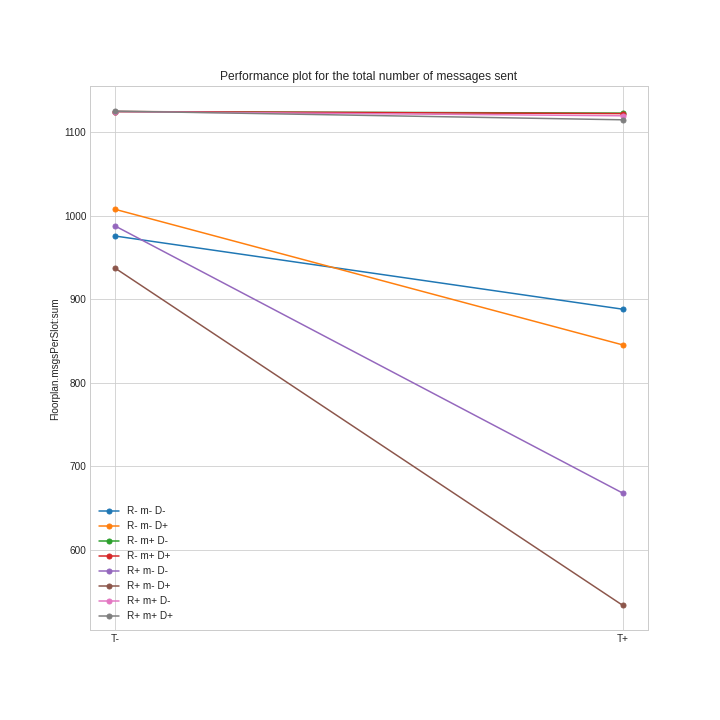
\includegraphics[width=\textwidth]{img/hd/messages-T-perfplot}
		\caption{Increase the size of the hear window when \(m\) is low
		to reduce the total number of messages
		sent}\label{subfig:hdperfmessagesT}
	\end{subfigure}
	\caption{Performance plots for the total number of messages
	sent}\label{fig:hdperfmessages}
\end{figure}

\subsubsection{Broadcast time}\label{subsubsec:hd2krtime}

Since in all the experiments we have always reached a coverage of at least
\(99\%\), here we will only discuss the broadcast time needed to reach the 99th
percentile of the coverage.

We have a large unexplained variation (\(7.95\%\)). The reason for this result
will be discussed in \chref{ch:starting-node}.

We can see that the most important factor is the broadcast radius that accounts
for the \(71.25\%\) of the variation, followed by the size of the hear window
(\(19.30\%\)). Other factors and their combinations are irrelevant. We note that
these variations are much larger than the unexplained variation, so we can still
say that they are significant. Of course, their \(95\%\) confidence intervals
also gets larger: (\(63.62\%\), \(79.30\%\)) for \(R\) and (\(15.43\%\),
\(23.59\%\)) for \(T\), but they do not include the zero.

This means that we can reduce the broadcast time by increasing the broadcast
radius to let the relayed messages to reach more user. Also the size of the hear
window can be decreased in order to reduce the time that each user wait before
deciding to relay or not relay the message. Of course, as stated before,
reducing the size of the hear window has a negative impact on the energy
efficiency, so some trade-off considerations are required.

We note that we have performed a \emph{logarithmic transformation of the
predicted variable} \idest{the total broadcast time} in order to meet the
assumption of finite variance for the residuals, as discussed in
\secref{subsec:hdassumptions}. This means that the final approximated regression
model for the broadcast time is transformed into the one shown
in~\eqref{eq:hdtimelogregressionmodel}, with \(R\) and \(T\) normalized between
\(-1\) and \(1\). (factors with low influence are removed; 95\% confidence
intervals are show in parenthesis).

\begin{equation}\label{eq:hdtimelogregressionmodel}
	\begin{cases}
		\log(t_B) = q_0 + q_R \cdot R + q_T \cdot T + e\\
		q_0 = 4.782874\\
		q_R = -0.462452 & (-0.487897, -0.437006)\\
		q_T = 0.240663 & (0.215217, 0.266109)
	\end{cases}
\end{equation}

We can then predict the total broadcast time using the formula shown
in~\eqref{eq:hdtimeregressionmodel}.

\begin{equation}\label{eq:hdtimeregressionmodel}
	t_B = e^{4.782874 - 0.462452 \cdot R + 0.240663 \cdot T}
\end{equation}

And the 95\% confidence interval as shown in~\eqref{eq:hdtimeregressionci}.

\begin{equation}\label{eq:hdtimeregressionci}
	\begin{cases}
		t^-_B = e^{4.782874 - 0.487897 \cdot R + 0.215217 \cdot T}\\
		t^+_B = e^{4.782874 - 0.437006 \cdot R + 0.266109 \cdot T}\\
	\end{cases}
\end{equation}


\subsection{Testing the assumptions}\label{subsec:hdassumptions}

The assumptions of normality, independency and finite variance must be verified
for the residuals of the observations. The complete analysis can be found in
\code{2kr-assumptions-tests.ipynb}.

\subsubsection{Normality}\label{subsubsec:rectassumptionsnormality}

In this case, we get worse results for normality compared to those obtained in
the other scenarios, with generally lower \(R^2\) and few outliers in collisions
and in messages, but we can say anyway that the normality assumption is
verified, except to the covered users, but since we do not study this index, we
do not need to get it verified.

\subsubsection{Independency}\label{subsubsec:hdassumptionsindependency}

Independency is assumed by the way we have conducted the experiments. Anyway,
the scatter plots do not show any trend.

\subsubsection{Finite variance}\label{rectassumptionsvariance}

In the collision and messages plots we haven't trends but the behaviour is
blockwise, as we can see for example in \figref{fig:recttimevariance} with
swinging results and also in this case the order of magnitude of the residual is
lower than the one of the average predicted response, so we can conclude that
the assumption of finite variance is still valid.

As for other scenarios, to verify the assumption for the residuals of the 99th
percentile of the total broadcast time we need to perform a logarithmic
transformation of the predicted variable. The result is shown in
\figref{fig:recttimevariance}.

\begin{figure}[htb]
	\centering
	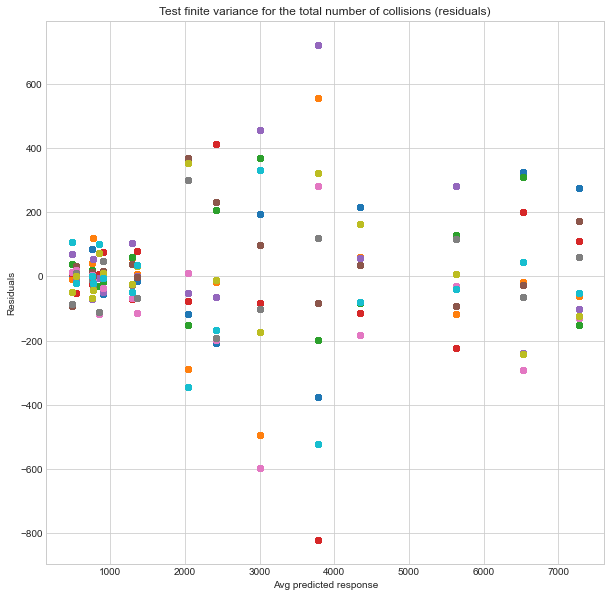
\includegraphics[width=0.6\textwidth]{img/rect/collisionvariance.png}
	\caption{Scatter plot of the variance of the residuals of the
	collisions. No trends but blockwise
	behaviour}\label{fig:recttimevariance}
\end{figure}



\section{Rectangular scenario}\label{sec:rectangular}

\subsection{2\texorpdfstring{\textsuperscript{k}}{k}r
analysis}\label{subsec:rect2kr}

Analysis performed with \(k\!=\!4\) and \(r\!=\!10\), for a total of \(2^4 \cdot
10 \!=\!160\) experiments. The performance indexes evaluated are the one defined
in \secref{sec:indexes}. When we talk about the total number of messages sent
remember that we are analyzing the \emph{energy efficiency} (\(\mathit{Eff}\))
of the network.

The simulation configuration for this analysis, named ``Rectangular2kr'' can be
found in the \code{simulations.ini} file. The simulations have been run using
our \code{simulate.sh} script with the following command:
\begin{verbatim}
$ ./simulate.sh -s Rectangular -c Rectangular2kr
\end{verbatim}

First, we have verified that the range of values for the \code{maxCopies}
parameter (3--7) was fine. The analysis can be found in \code{histograms.ipynb}.
Here, we just check that with \(m\!=\!3\) and \(m\!=\!7\) we get that a lot of
users decide to not relay the message in the first case and only a small bunch
of users decide to not relay the message in the second case.

Then, the 2\textsuperscript{k}r analysis can be found in \code{2kr.ipynb}. We
will verify the assumptions of normality, independence and finite variance for
the residuals in \secref{subsec:rectassumptions}. Here we will discuss the
results.

\section{Coverage}\label{sec:startnodecoverage}

File \code{coverage.ipynb} contains the histograms for the coverage obtained
with the configuration named ``StartNodePosition''. All parameters have been
fixed and we have performed 200 experiments with the starting user at the
center, border and corner --- for a total of 600 experiments.

The notebook also shows statistics about the coverage in the three cases.
Results are shown in \tableref{table:startnodecoveragestats}.

\begin{table}[hbt]
	\centering
	\begin{tabular}{lcccc}
		\toprule
		Start Node Pos\@. & Mean & Std\@. Dev\@. & Min\@. & Max\@. \\
		\midrule
		Center & \makecell[c]{\(1235.785\) \\ (\(98.942\%\))}
		       & \makecell[c]{\(7.084471\) \\ (\(0.5672\%\))}
		       & \makecell[c]{\(1213\) \\ (\(97.1177\%\))}
		       & \makecell[c]{\(1248\) \\ (\(99.9199\%\))} \\[16pt]
		Border & \makecell[c]{\(1225.345\) \\ (\(98.1061\%\))}
		       & \makecell[c]{\(123.317566\) \\ (\(9.8733\%\))}
		       & \(0\)
		       & \makecell[c]{\(1248\) \\ (\(99.9199\%\))} \\[16pt]
		Corner & \makecell[c]{\(910.64\) \\ (\(72.9095\%\))}
		       & \makecell[c]{\(546.580205\) \\ (\(43.7614\%\))}
		       & \(0\)
		       & \makecell[c]{\(1248\) \\ (\(99.9199\%\))} \\
		\bottomrule
	\end{tabular}
	\caption{Statistics about coverage when the starting node is in the
	center/border/corner (low density
	condition)}\label{table:startnodecoveragestats}
\end{table}

As we can see, the mean is higher if the starting user is positioned in the
center and lower if it is positioned in the border or corner. Additionally we
have higher standard deviations when the starting user is moved near the corner.
When the starting user is in the center, we have are able to guarantee a
coverage of at least \(97\%\) with \(R\!=\!25m\) in low density conditions,
while when the starting user is placed at the border or the corner the coverage
can drop down to zero.

Files \code{\{low,high\}-density-coverage.ipynb} contain the analysis of the
coverage in the two conditions (low density and high density) when the radius is
varied from very low values to high values. Data has been collected using the
configurations named ``StartNodePositionLowDensity'' and
``StartNodePositionHighDensity''.

\figref{subfig:ldstartnodecoverage} shows the results for the low density
case\footnote{For easier visualization, the Jupyter notebook also contains the
same data plotted in three different figures rather than with the center, border
and corner cases in the same plot.}. As we can see, in the ``center'' case the
mean coverage starts very high even with low values of \(R\): The minimum mean
is around \(1150\) (from a total of \(1249\) reachable users) and it stabilizes
near the value \(1240\) for \(R \ge 25m\).

\begin{figure}[hbt]
	\centering
	\begin{subfigure}[b]{0.49\textwidth}
		\centering
		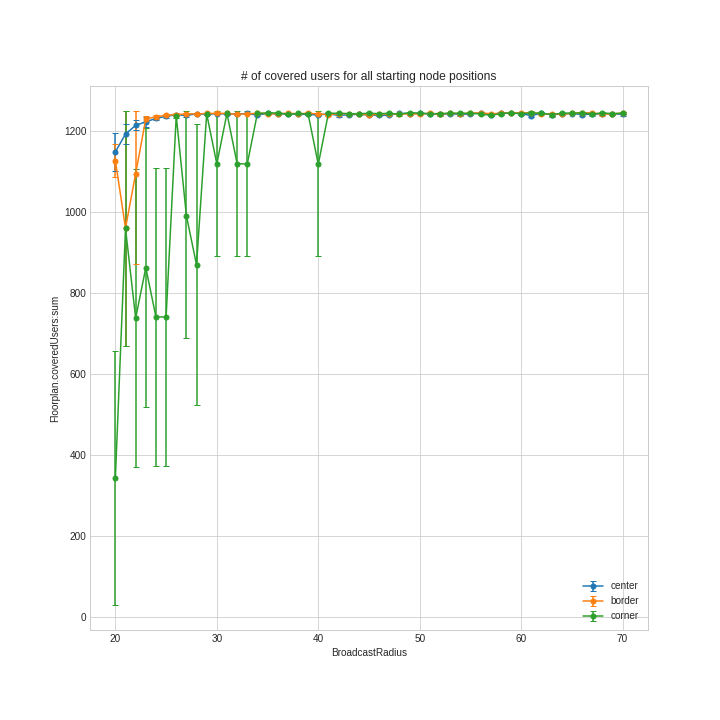
\includegraphics[width=\textwidth]{img/ld/start-node-coverage}
		\caption{Low density scenario}\label{subfig:ldstartnodecoverage}
	\end{subfigure}
	\begin{subfigure}[b]{0.49\textwidth}
		\centering
		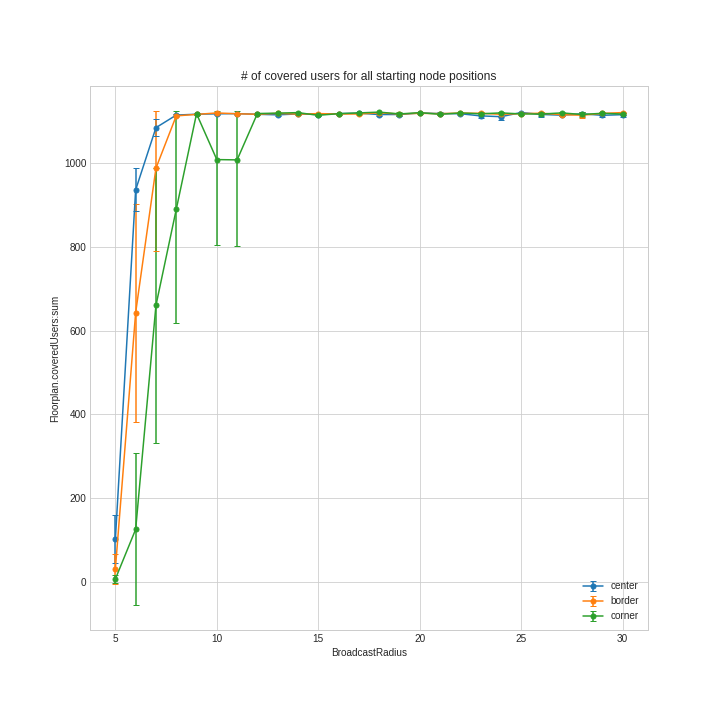
\includegraphics[width=\textwidth]{img/hd/start-node-coverage}
		\caption{High density
		scenario}\label{subfig:hdstartnodecoverage}
	\end{subfigure}
	\caption{For low values of \(R\), the coverage is generally worse if the
	starting node is in the corner rather than in the
	center}\label{fig:startnodepositioncoverage}
\end{figure}

Also in the ``border'' case the coverage stabilizes at high values with \(R \ge
25m\), but it has very high variance when the broadcast radius is very low and
it also happens that the first user sending the message is not able to reach
anyone, giving a coverage of zero.

In the ``corner'' case the situation is even worse: up until \(R \le 33m\) we
do not have a stable coverage and even after we get lower mean with a huge
variance with \(R\!=\!40m\). As we can see from the table at the end of the
notebook, this is due to a catastrophic experiment where the starting user has
not reached any user even with \(R\!=\!40m\).

\figref{subfig:hdstartnodecoverage} shows the results for the high density
scenario. Considerations are the same done for the low density scenario, so we
will not discuss the results here.

So, if possible, when designing a network of this type, to guarantee a nearly
perfect coverage, we should try to ensure that the starting user is near as much
as possible to the center or, at least, avoid the corners of the floorplan. If
this is not possible, to guarantee\footnote{With ``guarantee'' we do not mean a
100\% guarantee, of course: more experiments are needed to explore more
possibilities and, with the total randomness on the position of the users, the
only values of the broadcast radius that \emph{really} guarantees a coverage
greater than zero are those values that always make the starting user to reach
the entire floorplan immediately. Values found (\(40m\) and \(11m\)) are only an
\emph{hint} of minimum values that makes \emph{hard} to get a catastrophic
situation.} the coverage, it is necessary to increase the broadcast radius (\(R
> 40m\) for low density; \(R > 11m\) for high density).

The probability to found a user inside the area of reachability of the starting
node \idest{the probability to get a coverage greater than 0} can be easily
computed, in the general case, with~\eqref{eq:nocatastropheprobability}. The
equation has been derived by considering the inverse of the probability to found
\idest{the probability to \emph{not} found any node in the area of reachability,
which is the probability to found all the nodes in the area outside the area of
reachability} which is, for a single user, the area outside of the area of
reachability (\(X\cdot Y - \alpha\cdot\pi\cdot R^2\)) divided by the area of the
floorplan (\(X\cdot Y\)). This probability has been then extended to the case of
\(N\) users by raising it to the number of users except the first one (\(N-1\)).

\begin{equation}\label{eq:nocatastropheprobability}
	P = 1 - {\left(\frac{XY - \alpha\pi R^2}{XY}\right)}^{N-1}
\end{equation}

We can verify that for \(R\!=\!40m\), \(N\!=\!1250\), \(X\!=\!Y\!=\!500m\), with
the starting node in the corner (\(\alpha\!=\!\frac{1}{4}\)), we get:

\[
	P = 1 - {\left(\frac{500\cdot500 -
	\frac{1}{4}\pi\cdot40^2}{500\cdot500}\right)}^{1249} \simeq 99.81\%
\]

which is a quite high probability. Only in just \(\frac{1}{500}\) cases we will
get a coverage equal to zero in the case of the low density scenario with
\(R\!=\!40m\).

\subsubsection{Total number of collisions}\label{subsubsec:rect2krcollisions}

For the total number of collisions we get a very low unexplained variation
(\(0.72\%\)). The broadcast radius accounts for the \(64.31\%\) of the variation
and it is the dominant factor, as in other scenarios. As in the low density
scenario and differently from the high density one, the second most important
factor was the maximum number of copies, which accounts for the \(16.47\%\) of
the variation while the maximum relay delay (third factor) accounts only for the
\(4.86\%\) of the variation. In this case, also the combination of the broadcast
radius and the maximum number of copies is relevant (\(9.59\%\)). This results
are not surprisingly because the density of the rectangular scenario is the same
as the low density one (which is a square).

As in the case of other configurations, we need to decrease the broadcast radius
to reduce the total number of collision, which is an obvious consideration, and
as shown in \figref{fig:rectperfcollisionsm} using lower values for the maximum
number of copies reduces the total number of collisions.

The fact that the broadcast radius is less important in this scenario compared
to the high density case, but more important with respect to the low density,
can be explained by the fact that the users are scattered in the floorplan, so
we need a huger increase of the broadcast radius to see an effect, but they are
not so well distributed because they are flattened in the rectangle.

\begin{figure}[htb]
	\centering
	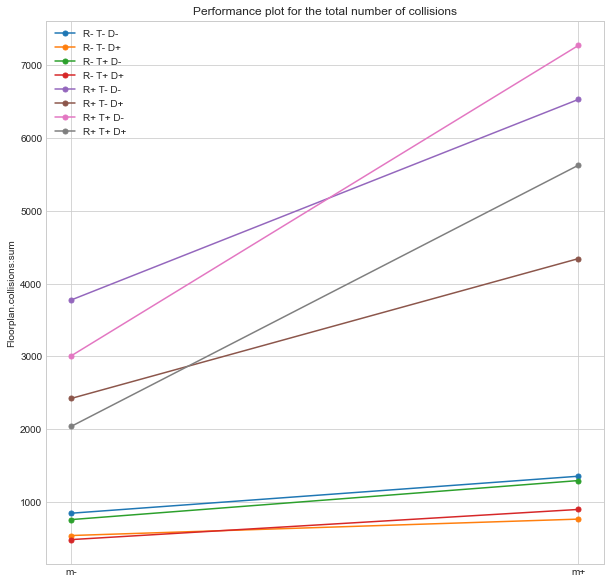
\includegraphics[width=\textwidth]{img/rect/collisions_m_perfplot.png}
	\caption{Decrease the maximum number of copies to decrease the total
	number of collisions}\label{fig:rectperfcollisionsm}
\end{figure}

\subsubsection{Total number of messages sent}\label{subsubsec:hd2krmessages}

This is an indication of the energy efficiency of the entire network.

The maximum number of copies is the dominant factor (\(85.98\%\)), as expected.
Also the broadcast radius \(R\) and its combination with the maximum
number of copies have a valuable impact on this index. The unexplained variation
is very low (\(0.53\%\)).

In \figref{subfig:hdperfmessagesm} we see that the total number of messages sent
decreases with an lower value of the \code{maxCopies} parameter, as expected.
We note that with \(m\!=\!6\) we get that nearly all the users of the network
relay the message. In \figref{subfig:hdperfmessagesR} we can see that less
messages are sent if an higher broadcast radius is used when \(m\!=\!2\). So,
with a low \(m\), we can further decrease the total number of messages sent by
increasing \(R\). Of course increasing the broadcast radius is not good for our
purpose to optimize the energy efficiency of the network, but as we can see from
\figref{subfig:hdperfmessagesT}, the same consideration made for \(R\) are also
valid for the hear window size \(T\). We perhaps expect \(T\) to hugely affect
the total broadcast time, so the selection of the factor \(T\) is a trade-off
between the energy efficiency and the total broadcast time.

\begin{figure}[hbt]
	\centering
	\begin{subfigure}[b]{0.33\textwidth}
		\centering
		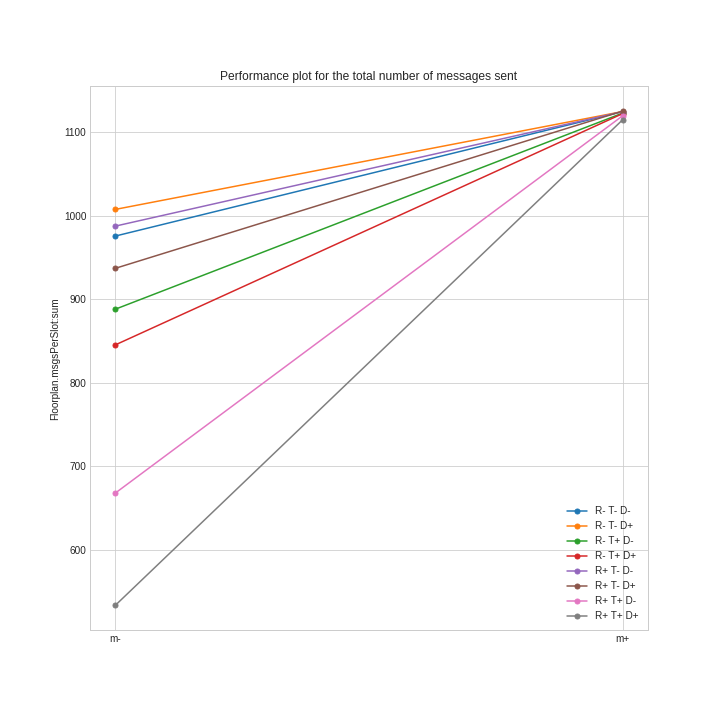
\includegraphics[width=\textwidth]{img/hd/messages-m-perfplot}
		\caption{When the maximum number of copies is reduced the total
		number of messages sent decreases}\label{subfig:hdperfmessagesm}
	\end{subfigure}
	\begin{subfigure}[b]{0.33\textwidth}
		\centering
		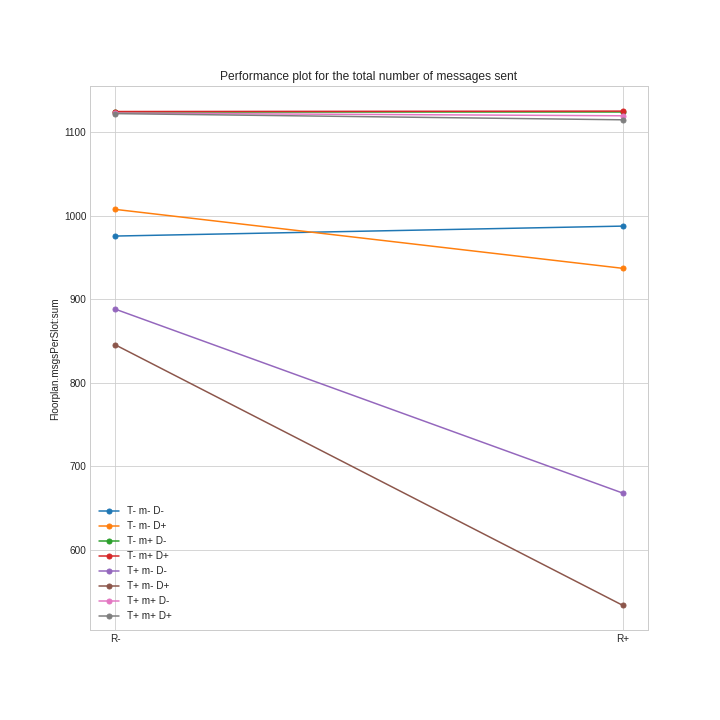
\includegraphics[width=\textwidth]{img/hd/messages-R-perfplot}
		\caption{Increase the broadcast radius when \(m\) is low to
		reduce the total number of messages
		sent}\label{subfig:hdperfmessagesR}
	\end{subfigure}
	\begin{subfigure}[b]{0.32\textwidth}
		\centering
		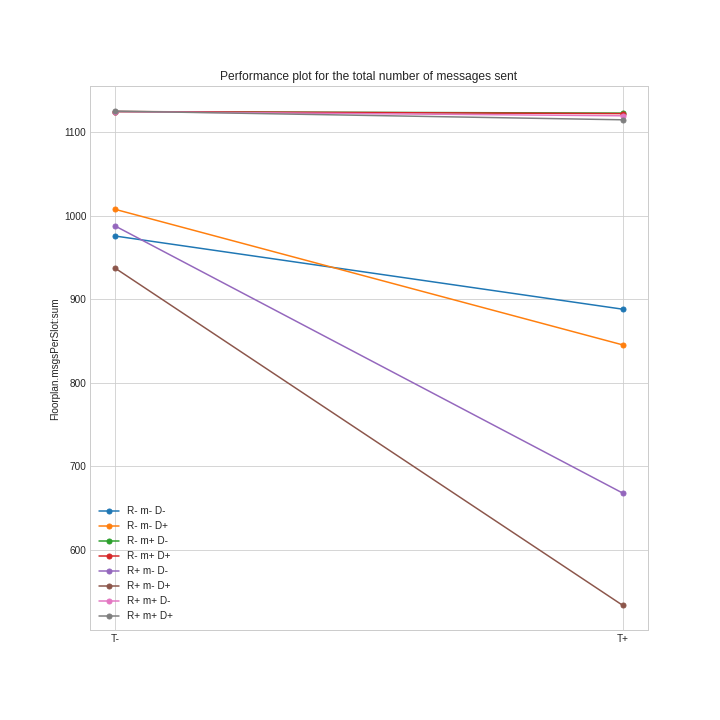
\includegraphics[width=\textwidth]{img/hd/messages-T-perfplot}
		\caption{Increase the size of the hear window when \(m\) is low
		to reduce the total number of messages
		sent}\label{subfig:hdperfmessagesT}
	\end{subfigure}
	\caption{Performance plots for the total number of messages
	sent}\label{fig:hdperfmessages}
\end{figure}

\subsubsection{Broadcast time}\label{subsubsec:hd2krtime}

Since in all the experiments we have always reached a coverage of at least
\(99\%\), here we will only discuss the broadcast time needed to reach the 99th
percentile of the coverage.

We have a large unexplained variation (\(7.95\%\)). The reason for this result
will be discussed in \chref{ch:starting-node}.

We can see that the most important factor is the broadcast radius that accounts
for the \(71.25\%\) of the variation, followed by the size of the hear window
(\(19.30\%\)). Other factors and their combinations are irrelevant. We note that
these variations are much larger than the unexplained variation, so we can still
say that they are significant. Of course, their \(95\%\) confidence intervals
also gets larger: (\(63.62\%\), \(79.30\%\)) for \(R\) and (\(15.43\%\),
\(23.59\%\)) for \(T\), but they do not include the zero.

This means that we can reduce the broadcast time by increasing the broadcast
radius to let the relayed messages to reach more user. Also the size of the hear
window can be decreased in order to reduce the time that each user wait before
deciding to relay or not relay the message. Of course, as stated before,
reducing the size of the hear window has a negative impact on the energy
efficiency, so some trade-off considerations are required.

We note that we have performed a \emph{logarithmic transformation of the
predicted variable} \idest{the total broadcast time} in order to meet the
assumption of finite variance for the residuals, as discussed in
\secref{subsec:hdassumptions}. This means that the final approximated regression
model for the broadcast time is transformed into the one shown
in~\eqref{eq:hdtimelogregressionmodel}, with \(R\) and \(T\) normalized between
\(-1\) and \(1\). (factors with low influence are removed; 95\% confidence
intervals are show in parenthesis).

\begin{equation}\label{eq:hdtimelogregressionmodel}
	\begin{cases}
		\log(t_B) = q_0 + q_R \cdot R + q_T \cdot T + e\\
		q_0 = 4.782874\\
		q_R = -0.462452 & (-0.487897, -0.437006)\\
		q_T = 0.240663 & (0.215217, 0.266109)
	\end{cases}
\end{equation}

We can then predict the total broadcast time using the formula shown
in~\eqref{eq:hdtimeregressionmodel}.

\begin{equation}\label{eq:hdtimeregressionmodel}
	t_B = e^{4.782874 - 0.462452 \cdot R + 0.240663 \cdot T}
\end{equation}

And the 95\% confidence interval as shown in~\eqref{eq:hdtimeregressionci}.

\begin{equation}\label{eq:hdtimeregressionci}
	\begin{cases}
		t^-_B = e^{4.782874 - 0.487897 \cdot R + 0.215217 \cdot T}\\
		t^+_B = e^{4.782874 - 0.437006 \cdot R + 0.266109 \cdot T}\\
	\end{cases}
\end{equation}



